\documentclass[11pt,xcolor=svgnames]{beamer}
\usepackage{dsfont,natbib,setspace,changepage,multirow}
\mode<presentation>

% replaces beamer foot with simple page number
\setbeamertemplate{navigation symbols}{}
%\setbeamerfont{frametitle}{series=\bfseries}
\setbeamercolor{frametitle}{fg=Black}

\setbeamertemplate{footline}{
   \raisebox{5pt}{\makebox[\paperwidth]{\hfill\makebox[20pt]{\color{gray}\scriptsize\insertframenumber}}}}

\graphicspath{{/Users/mtaddy/Dropbox/inputs/}}
\usepackage{algorithm}
\usepackage{algorithmic}

% colors
\newcommand{\theme}{\color{Maroon}}
\newcommand{\bk}{\color{black}}
\newcommand{\rd}{\color{DarkRed}}
\newcommand{\fg}{\color{ForestGreen}}
\newcommand{\bl}{\color{blue}}
\newcommand{\gr}{\color{black!50}}
\newcommand{\sg}{\color{DarkSlateGray}}
\newcommand{\nv}{\color{Navy}}
\setbeamercolor{itemize item}{fg=gray}

% common math markups
\newcommand{\bs}[1]{\boldsymbol{#1}}
\newcommand{\mc}[1]{\mathcal{#1}}
\newcommand{\mr}[1]{\mathrm{#1}}
\newcommand{\bm}[1]{\mathbf{#1}}
\newcommand{\ds}[1]{\mathds{#1}}
\newcommand{\indep}{\perp\!\!\!\perp}
\def\plus{\texttt{+}}
\def\minus{\texttt{-}}

% spacing and style shorthand
\setstretch{1.1}

\begin{document}

\setcounter{page}{0}
{ \usebackgroundtemplate{
\includegraphics[height=\paperheight]{phoenix}}
\begin{frame}[plain]
\begin{center}

{\bf \LARGE \theme }

{\bf \Large  Big Data and Bayesian Nonparametrics}

\vskip 2cm
Matt Taddy,  Chicago Booth


\vskip .25cm
{\texttt{faculty.chicagobooth.edu/matt.taddy/research}}

\end{center}
\end{frame} }


\begin{frame}

{\bf Big Data}


\vskip .5cm
{\nv The data are super weird.  }
\begin{itemize}
\item Internet transaction data distributions have a big spike at zero and spikes at other discrete values (e.g., 1 or \$99).
\item Big tails (e.g., \$12 mil/month eBay user spend) that matter.
\item We cannot  write down believable models.
\end{itemize}

\vskip .25cm
{\nv The sample sizes are enormous.}
\begin{itemize}
\item we'll see 21 and 200 million today.  
\item Data can't fit in memory, or even storage, on a single machine.
\item Our familiar MCMC algorithms take too long.
\end{itemize}

\end{frame}

\begin{frame}

Both `Big' and `Strange' beg for nonparametrics.

\vskip .5cm
In usual BNP you {\it model} a complex generative process with flexible priors, then apply that model directly in prediction and inference.
\[
\text{e.g.,~~~}y = f(\bm{x}) + \epsilon,~~\text{or~even~just}~~f(y|\bm{x})
\]
However averaging over all of the nuisance parameters we introduce to be `flexible' is a hard computational problem.

\vskip .5cm
\hfill {\theme Can we do scalable BNP?}
\end{frame}

\begin{frame}

Frequentists are great at finding simple procedures {\gr\small (e.g. $[\bm{X}'\bm{X}]^{-1}\bm{X}'y$)\!} and  showing that they will `work' regardless of the true DGP.

\hfill{\gr \small (DGP = Data Generating Process)~~~~~~~}

\vskip .5cm
This is classical `distribution free' nonparametrics.

\vskip .15cm
1: Find some statistic that is useful regardless of DGP.

\vskip .15cm
2: Derive the distribution for this stat under minimal assumptions.

\vskip .5cm
Practitioners apply the simple stat and feel happy that it will work.

\vskip .2cm
No need to re-model the underlying DGP each time, and you \\don't need to have a PhD in Bayesian Statistics to apply the ideas.

\vskip .5cm\hfill
{\theme Can we Bayesians provide something like this?}

\end{frame}

\begin{frame}

{\bf distribution free Bayesian nonparametrics}

\vskip .5cm
{Find some {\it statistic of the DGP} that you care about.}
\vskip .1cm
\begin{itemize}
\item Derive it from first principles, e.g. moment conditions.
\item Or a statistic could be an algorithm that we know works.
\end{itemize}
\vskip .1cm
Call this statistic $\bs{\theta}(g)$ where $g(\bm{z})$ is the DGP (e.g., for $\bm{z} = [\bm{x},y]$).

\vskip .5cm
Then you write down a flexible  model for the DGP $g$, and study properties of the posterior on $\bs{\theta}(g)$ induced by the posterior over $g$.

\end{frame}

\begin{frame}

{\bf A flexible model for the DGP}
\begin{equation*}
g(\bm{z}) = \frac{1}{|\bs{\theta}|}\sum_{l=1}^L \theta_l \ds{1}{[\bm{z} =
\bs{\zeta}_l]}, ~~~ \theta_l/|\bs{\theta}| \stackrel{iid}{\sim} \mr{Dir}(a)\end{equation*}

\vskip .25cm
After observing $\bm{Z} = \{\bm{z}_1 \ldots \bm{z}_n\}$, posterior has $\theta_l \sim \mr{Exp}(a\!+\!\ds{1}_{\bs{\zeta}_l \in \bm{Z}})$. {\gr (say every $\bm{z}_i = [\bm{x}_i,y_i]$ is unique)}.

\vskip .5cm
$a \to 0$ leads to $\mr{p}(\theta_l = 0) = 1$ for $\bs{\zeta}_l \notin \bm{Z}$.
\[
\Rightarrow g(\bm{z}\mid\bm{Z}) = \tfrac{1}{|\bs{\theta}|}
\sum_{l=1}^L \theta_l \ds{1}{[\bm{z} =
\bm{z}_l]},~~~\theta_i \sim \mr{Exp}(1)
\]

\hfill
{This is just the Bayesian bootstrap.}

\hfill {\gr Ferguson 1973, Rubin 1981}

\end{frame}

\begin{frame}

{\bf {\gr Example: } Ordinary Least Squares}

\vskip .5cm
{\it Population} OLS is a posterior functional
\begin{equation*}
\bs{\beta} = (\bm{X}'\bs{\Theta}\bm{X})^{-1}  \bm{X}'\bs{\Theta}\bm{y}
\end{equation*}
where $\bs{\Theta} = \mr{diag}(\bs{\theta})$.  
{\theme This is a random variable. \gr (sample via BB)}

\vskip .75cm
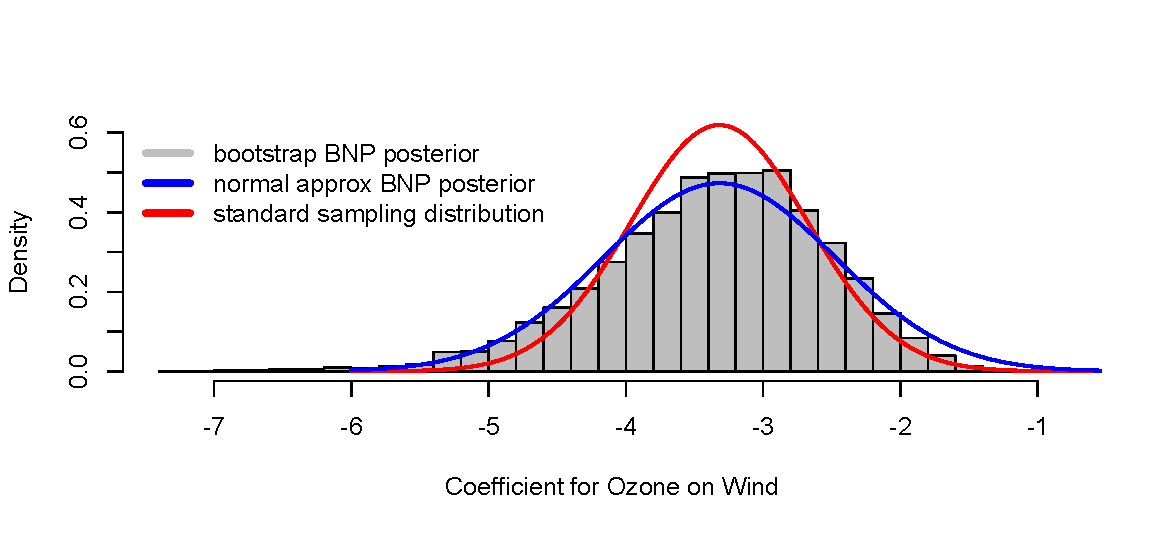
\includegraphics[width=\textwidth]{graphs/ozone}
\end{frame}

% \begin{frame}[fragile]

% {\footnotesize\gr
% \begin{verbatim}
% data(airquality); n <- nrow(airquality)
% B <- 1000; beta <- vector(length=B)
% for(b in 1:B){
%   fit <- lm(Ozone ~., data=airquality, weights=rexp(n))
%   beta[b] <- coef(fit)["Wind"] }
% sampfit <- lm(Ozone ~ ., data=airquality)
% coef <- summary(sampfit)$coef["Wind",1:2]
% x <- as.matrix(cbind(1,na.omit(airquality)[,-1]))
% xxi <- solve(crossprod(x))
% sandwich <- xxi%*%t(x)%*%diag(sampfit$resid^2)%*%x%*%xxi
% hist(beta, col=8, main="", 
%   xlab="Coefficient for Ozone on Wind", 
%   freq=FALSE,ylim=c(0,0.6),breaks=25)
% grid <- seq(-6,5,length=500)
% lines(grid, dnorm(grid,coef[1],coef[2]),col=2,lwd=2)
% lines(grid, dnorm(grid,coef[1],sqrt(sandwich[3,3])),col=4,lwd=2)
% legend("topleft",col=c(8,2),lwd=4, 
%   legend=c("bootstrap BNP posterior",
%            "normal approx BNP posterior",
%            "standard sampling distribution"),bty="n")
% \end{verbatim}
% }

% \end{frame}

\begin{frame}

{\nv \bf What is the blue line? } \\BB sampling is great, but analytic approximations are also useful.

\vskip .5cm
Consider a first-order Taylor series approximation,
\[
\bs{\tilde \beta} = [\bm{X}'\bm{X}]^{-1}\bm{X}'y + 
\nabla \bs{\beta}\big |_{\bs{\theta}=\bm{1}} (\bs{\theta} - \bm{1})
\]

We can derive {\it exact} posterior moments for $\bs{\tilde \beta}$ under $\theta_i \stackrel{iid}{\sim}\mathrm{Exp}(1)$.

\vskip .25cm
e.g., $\mr{var}(\bs{\tilde \beta}) \approx (\bm{X}^{\prime}\bm{X})^{-1}\bm{X}^{\prime}\mr{diag}(\bm{e})^2\bm{X}^{\prime}(\bm{X}^{\prime}\bm{X})^{-1}$, where $e_i  = y_i - \bm{x}_i'\bs{\hat\beta}$.

\vskip .25cm
This is the familiar Huber-White `Sandwich' variance formula.

\vskip .25cm{\gr \hfill
 See Lancaster 2003 or Poirier 2011.}

\end{frame}

\begin{frame}

{\bf{\gr Example:} User-Specific Behavior in Experiments}

\vskip .5cm
{\nv eBay runs lots of experiments:} they make changes to the marketplace (website) for random samples of users.

\vskip .5cm
Every experiment has response $y$ and treatment $d$ {\gr [0/1]}.

\vskip .5cm
We know $\bm{x}_i$ about user $i$.

\vskip .2cm
\begin{itemize}
\item Their previous spend, items bought, items sold...
\item Page view counts, items watched, searches, ...
\item All of the above, broken out by product, fixed v. auction, ...
\end{itemize}

\vskip .25cm
$\bm{x}_i$ are  possible sources of heterogeneity. About 400 in our example.

\end{frame}

\begin{frame}

What is `heterogeneity in treatment effects'? {\gr(HTE)}

\vskip .5cm Different units {\gr [people, devices]} respond differently to some treatment you apply {\gr [change to website, marketing, policy]}.  

\vskip .5cm I imagine it exists.  

\vskip .5cm Can we accurately measure heterogeneity: index it on $\bm{x}$?

\end{frame}


\begin{frame}

In our illustrative example,
$d_i$ = bigger pictures in my eBay.

\vskip .25cm
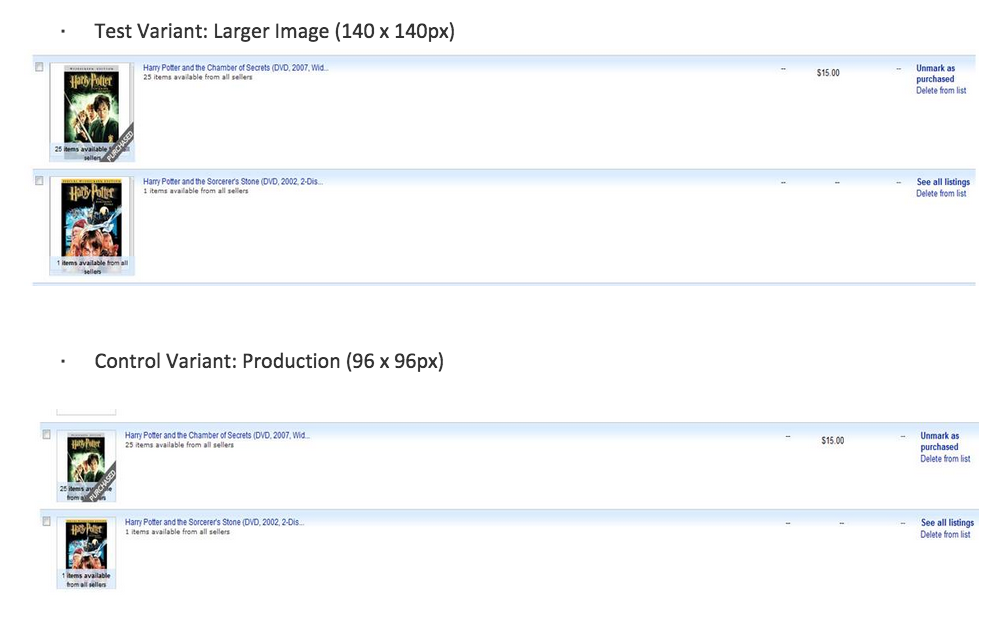
\includegraphics[width=4.5in]{graphs/userex}

21 million tracked visitors over 5 weeks, 2/3 in treatment.
\vskip -.5cm

\end{frame}


\begin{frame}

{\theme a statistic we care about ...}

\vskip .25cm
Potential outcome: $\upsilon_{i}({\sf d})$ is $\approx$ \$ for user
$i$ under  ${\sf d}$.  

\vskip .05cm
We only ever get to see one of $\upsilon_{i}({\sf t})$ and $\upsilon_{i}({\sf c})$: `y'.

\vskip .25cm
We care about `$\bs{\gamma}$' from the {\it moment condition}
\[
\ds{E}\left[\bm{x}(\upsilon({\sf t}) - \upsilon({\sf c})-\bm{x}'\bs{\gamma})\right] = \bs{0} 
\]
This says $\bm{x}'\bs{\gamma}$ is uncorrelated with the treatment effect $\upsilon({\sf t}) - \upsilon({\sf c})$.

\vskip .25cm
Since randomization implies that $\ds{E}[\bm{x}\upsilon({\sf d})] = \ds{E}[\bm{x}\upsilon({\sf d}) | d]$, we get
\[
\bs{\gamma} = 
\ds{E}\left[\bm{x}\bm{x}'\right]^{-1}
\bigg(\ds{E}[\bm{x}y | {\sf d} = {\sf t}] - \ds{E}[\bm{x}y|  {\sf d} = {\sf c}]\bigg)
\]

\end{frame}


\begin{frame}

As we did with OLS, consider a first-order approximation
\begin{equation*}
\bs{\tilde \gamma} = \bs{\hat \gamma} + 
\nabla \bs{\gamma}\big|_{\bs{\theta}=\bm{1}} (\bs{\theta} - \bm{1}).
\end{equation*}
where
\[
\bs{\hat \gamma} = \bs{\gamma}\big|_{\bs{\theta}=\bm{1}} = n(\bm{X}'\bm{X})^{-1}
 \left(\frac{\bm{X}_{\sf t}'\bm{y}_{\sf t}}{n_{\sf t}} - 
 \frac{\bm{X}_{\sf c}'\bm{y}_{\sf c}}{n_{\sf c}}\right).
\]

This yields an approximate variance
\[
\mathrm{var}(\bs{\tilde\gamma}) \approx (\bm{X}'\bm{X})^{-1}\bm{X}'
\mathrm{diag}(\bs{e}^\star)
\bm{X}(\bm{X}'\bm{X})^{-1}
\]
with `treatment effect residuals' 
\[
 e^\star_i = \left( \frac{\ds{1}_{[i\in {\sf t}]}}{n_{\sf t}} - \frac{\ds{1}_{[i\in {\sf c}]}}{n_{\sf c}}\right)ny_i -\bm{x}_i'\bs{\hat\gamma}.
\] 

\gr \hfill Or you can bootstrap, but it takes a long time.
\end{frame}

\begin{frame}

e.g., coefficient on purchase within last-year vs an intercept:

\vskip .25cm
{\footnotesize\it
\gr million users:~~~~~~~~~~~~~~~7.45~~~~~~~~~~~~~~~~~~~~~~10.97~~~~~~~~~~~~~~~~~~~~~13.22}
\begin{center}
\vskip -.5cm
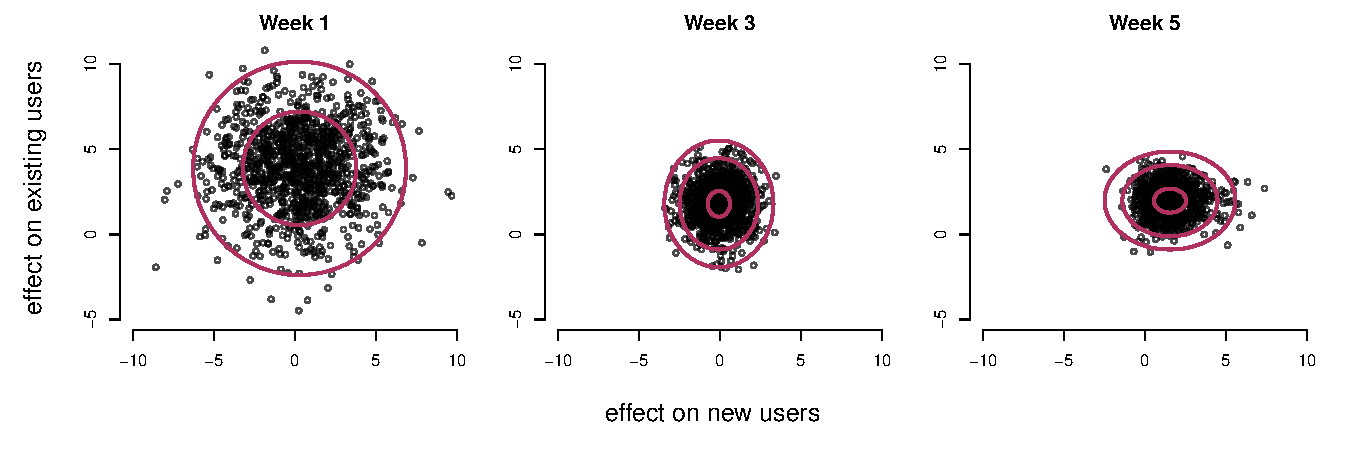
\includegraphics[width=.9\textwidth]{graphs/gammapost}
\end{center}

\vskip .25cm
{\gr Sample is from posterior, contours are normal approximation.}

{This is a statistic we care about}, even if the truth is nonlinear.

\vskip -.5cm
\end{frame}

\begin{frame}


{\bf {\gr Example:} Decision Trees}

\vskip .5cm
Trees are great: nonlinearity, deep interactions, heteroskedasticity.

\begin{center}
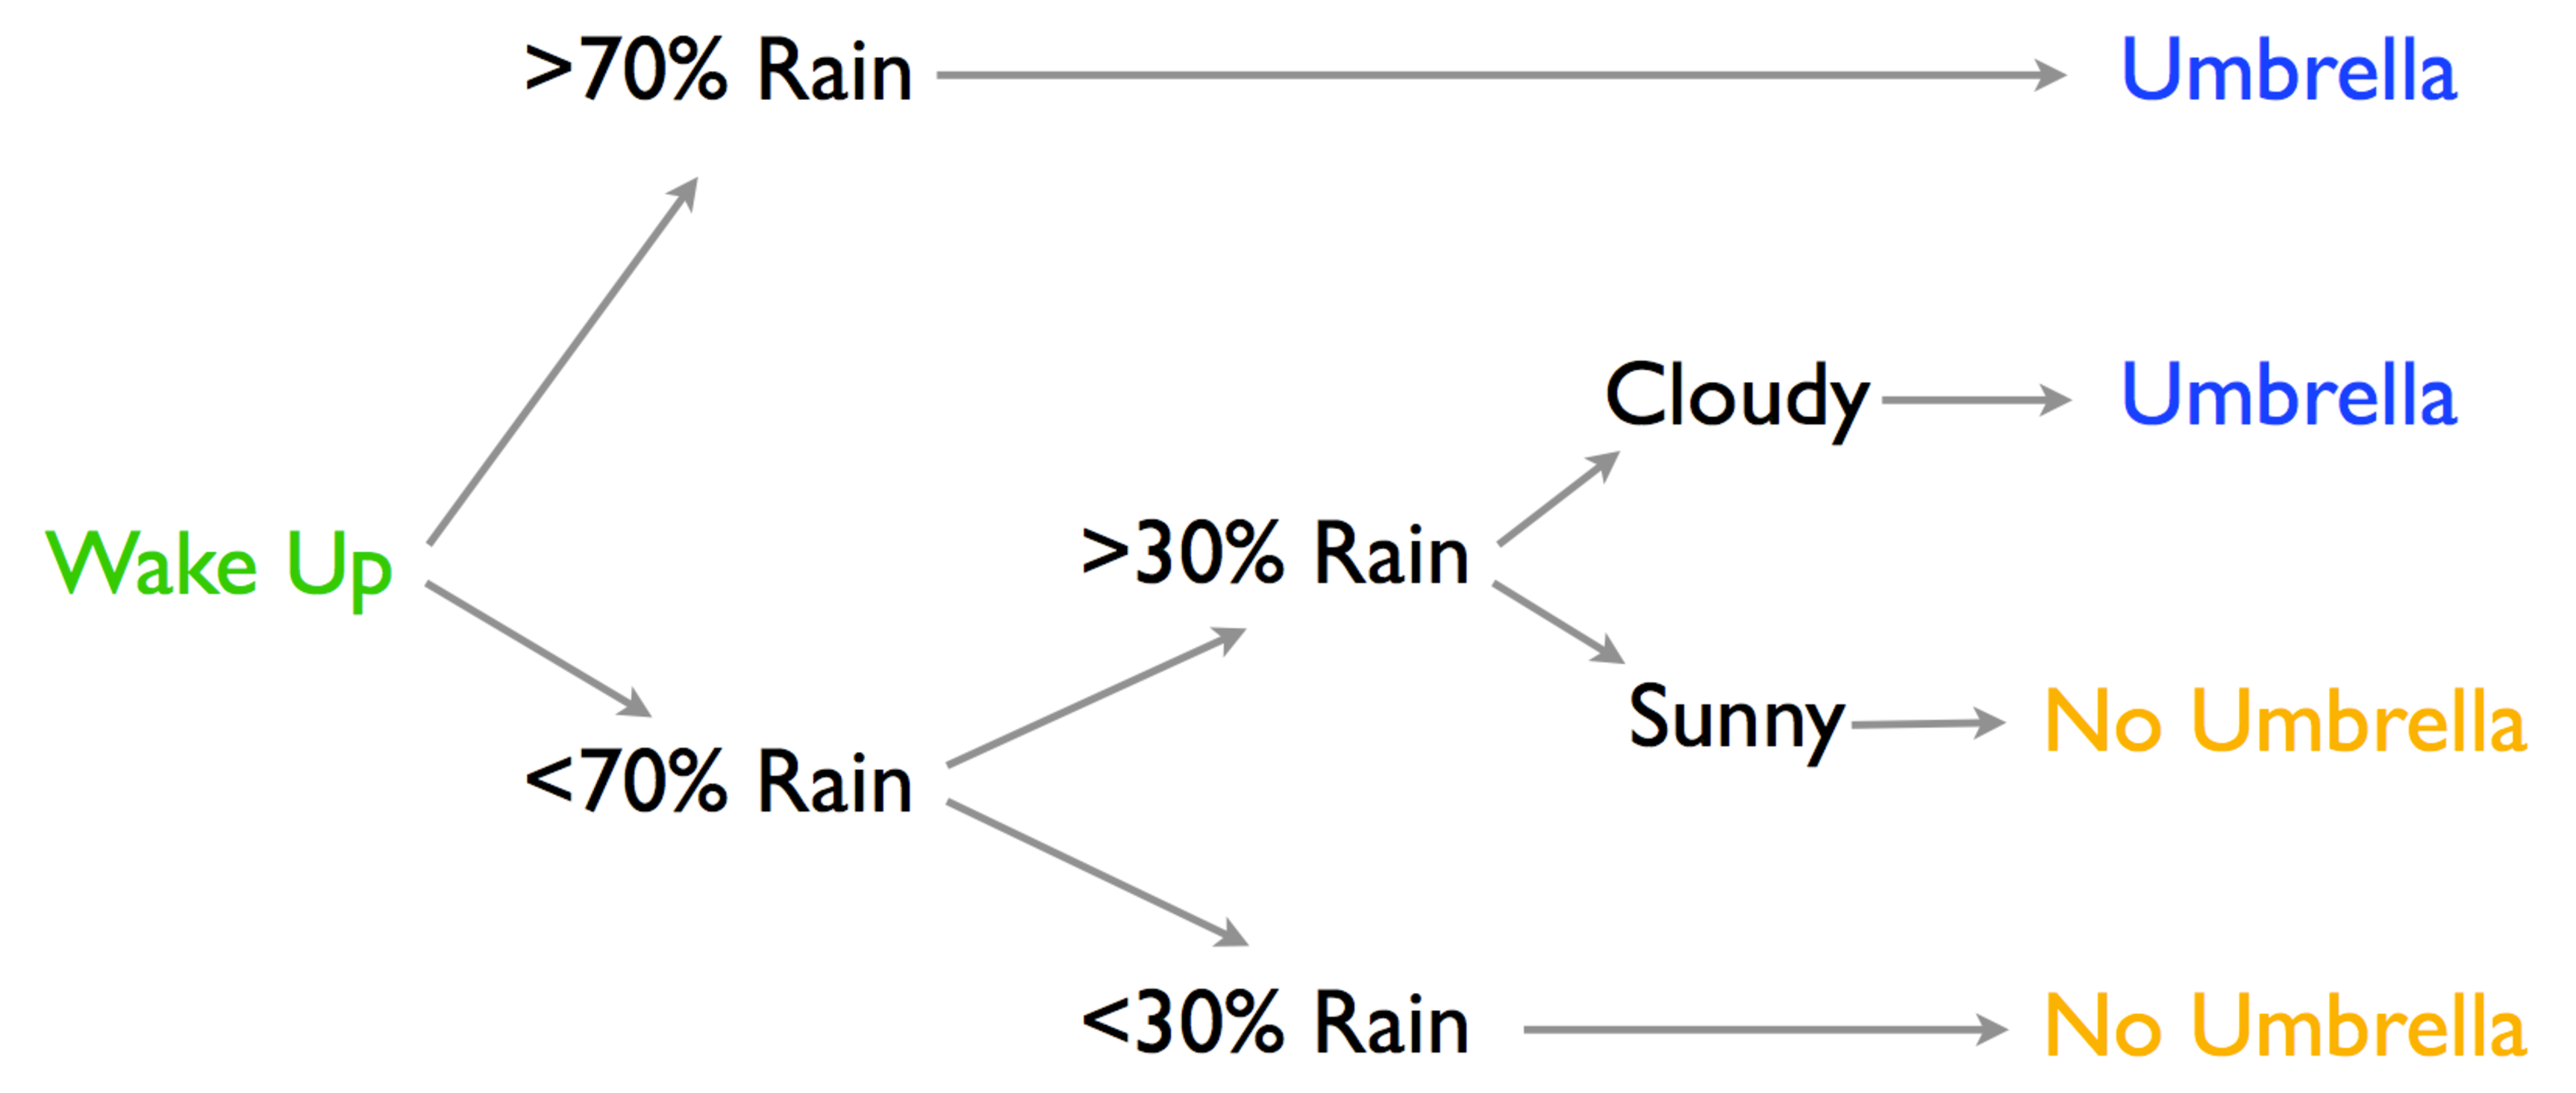
\includegraphics[width=4in]{../graphs/umbrella}
\end{center}

The `optimal' decision tree is a statistic we care about {\gr (s.w.c.a)}.


\end{frame}


\begin{frame}


{\bf {\theme CART:} greedy growing with optimal splits}

\vskip .5cm
Given node $\{\bm{x}_i,y_i\}_{i=1}^n$ and DGP weights $\bs{\theta}$,
find $x$ to minimize 
\begin{align*}
|\bs{\theta}|\sigma^2(x, \bs{\theta} ) &= \sum_{k \in \mathrm{left}(x)} \theta_k (y_k - \mu_{\mathrm{left}(x)})^2 \\&+ \sum_{k \in \mathrm{right}(x)} \theta_k (y_k - \mu_{\mathrm{right}(x)})^2
\end{align*}
for a regression tree.  Classification impurity can be Gini, etc.


\vskip .5cm
Population-CART might be a statistic we care about.


\vskip .1cm{\gr 
Or, in settings where greedy CART would do poorly (big $p$), \\a randomized splitting algorithm might be a better s.w.c.a.}



\end{frame}


\begin{frame}[fragile]

{\bf \theme Bayesian Forests: \bk a posterior for CART trees}

\vskip .25cm
For $b=1 \dots B$: \\
   ~~~~~~~~~~$\bullet$ draw $\boldsymbol{\theta}^b \stackrel{iid}{\sim} \mathrm{Exp}(\mathbf{1})$
   \\
   ~~~~~~~~~~$\bullet$ run weighted-sample CART to get $\mathcal{T}_b = \mathcal{T}(\boldsymbol{\theta}^b)$
 
\vskip .5cm\small 
~~~~~~~~~~~~~~~~~~~~~{\it one tree~~~~~~~~~~~~~~~~~~~~~~~~~~~~~~~~~~posterior mean}\\

\includegraphics[height=1.75in]{../../bayesian-forest/graphs/MCtreedraw}   
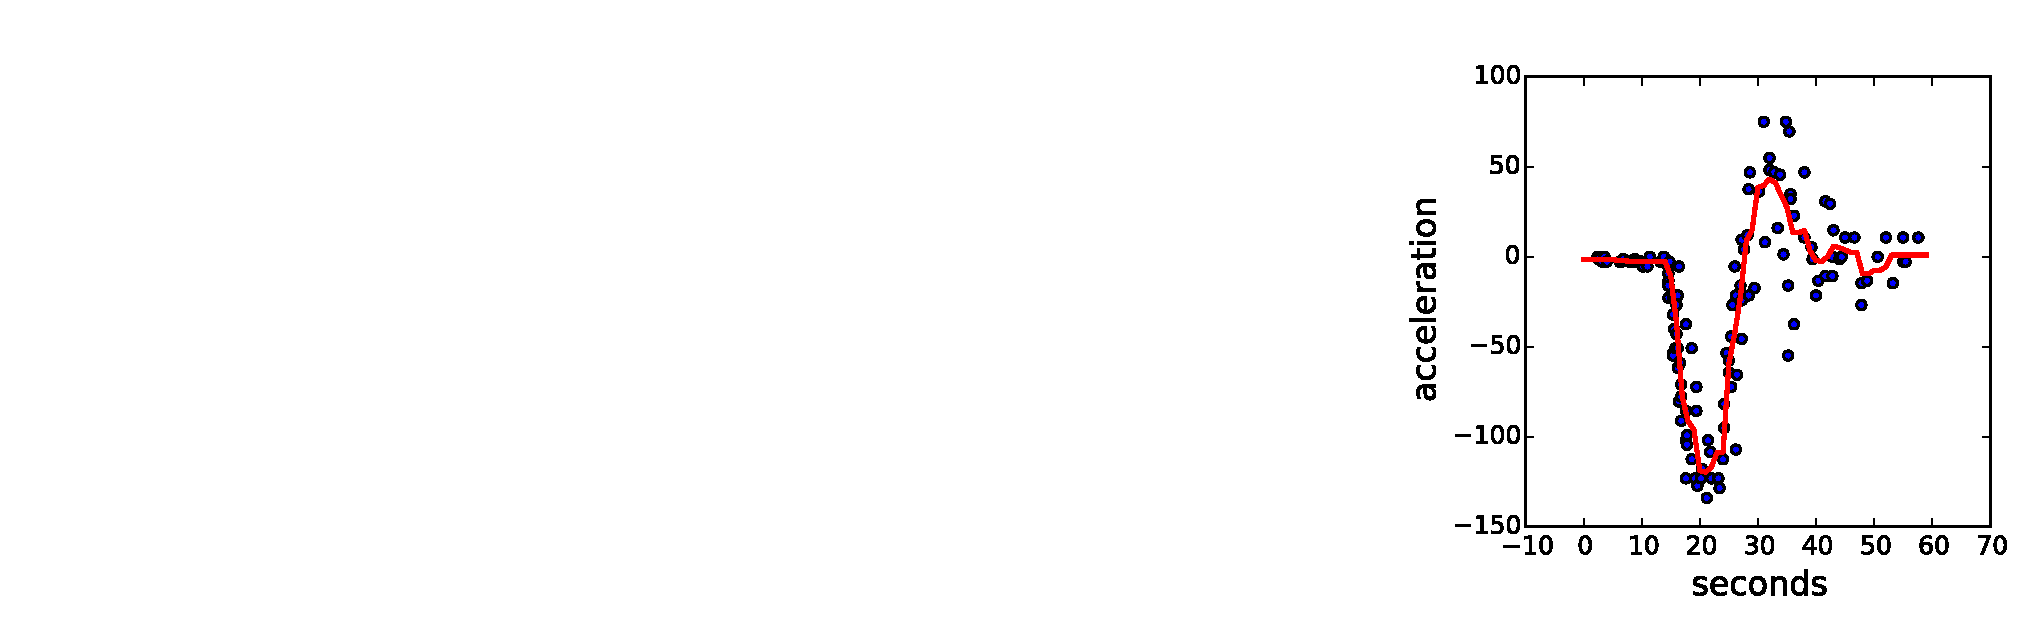
\includegraphics[height=1.75in]{../../bayesian-forest/graphs/MCbforest}   

\vskip .25cm{
Random Forest $\approx$ Bayesian forest $\approx$ posterior over CART fits.}

\vskip -.5cm

\end{frame}


\begin{frame}

{\bf Treatment Effect Trees}

\vskip .35cm
Athey\texttt{+}Imbens propose indexing user HTE by fitting CART to
\[
y^\star_i = y_i \frac{d_i - q}{q(1-q)} = \left\{
\begin{array}{cc}
y_i/(1-q) &\text{if~} d_i=0\\
y_i/q &\text{if~} d_i=1
\end{array}\right.
\]
where $q$ is the probability of treatment ($2/3$ in our example).

\vskip .35cm
This works because
\[
\ds{E}[y^\star_i | \bs{\upsilon}_i] = 
%q \upsilon_i(1)\frac{1 - q}{q(1-q)} - (1-q) \upsilon_i(0)\frac{q}{q(1-q)}
\upsilon_i(1)- \upsilon_i(0)
\]
where $\upsilon_i(d)$ is the potential outcome for user $i$ if $d_i = d$.\\  {\gr We only get to observe one of these: $y_i =
\upsilon_i(d_i)$.}

\end{frame}

\begin{frame}

We can apply the Bayesian bootstrap (i.e., fit a BF) to assess \\{\it posterior uncertainty} about these treatment-effect trees.

\vskip .15cm
e.g., sample depth-5 CART with min-leaf-size-$10^5$ after one week:
\begin{center}
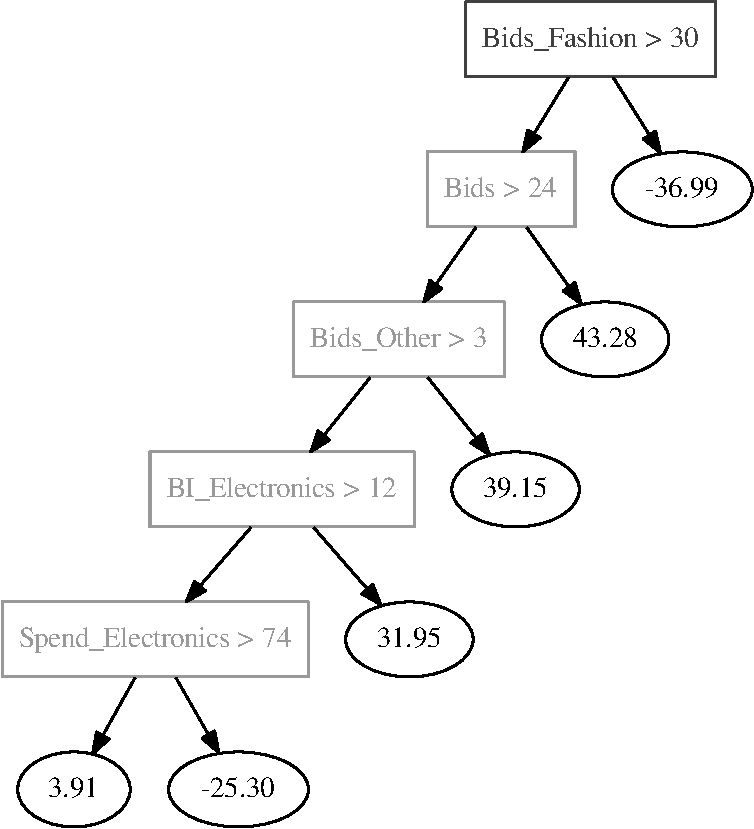
\includegraphics[width=.5\textwidth]{graphs/samptree_week1}
\end{center}
\hfill prob variable is node in tree: {\color{black!50} $\mr{p} <\tfrac{1}{3}$},
{\color{black!75}  $\mr{p} \in
\left[\tfrac{1}{3},\tfrac{1}{2}\right)$}, and {\color{DarkRed}  $\mr{p}
\geq \tfrac{1}{2}$}.
\end{frame}

\begin{frame}

After 5 weeks the tree is much more stable.
\begin{center}
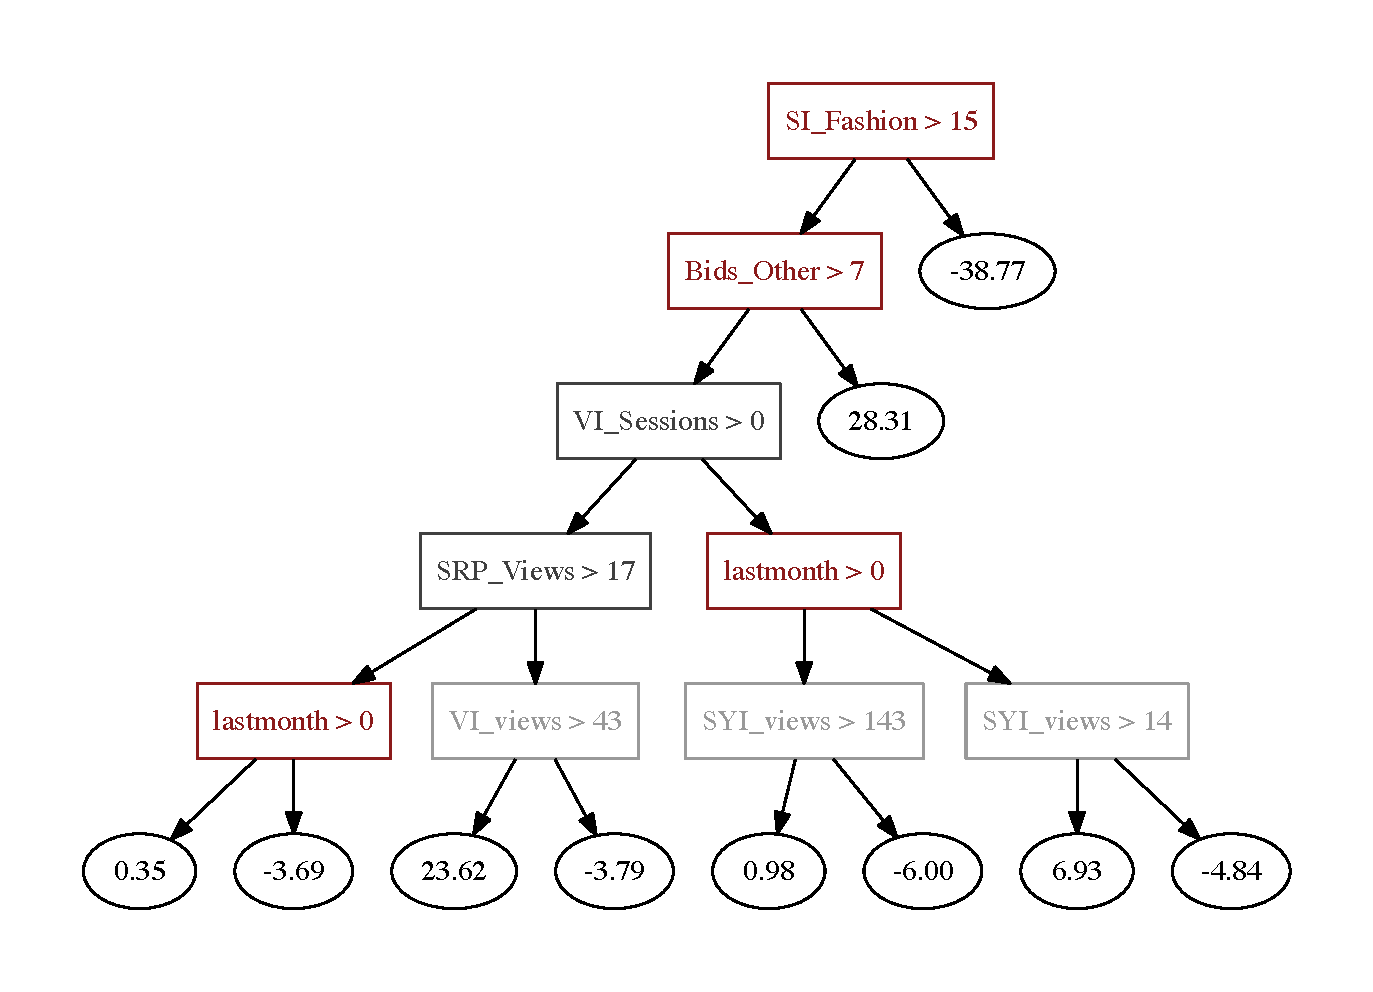
\includegraphics[width=.9\textwidth]{graphs/samptree_week5}
\end{center}

\end{frame}

\begin{frame}

We can quantify uncertainty about all sorts of structure.

\vskip .5cm
{\bf Posterior probability of CART splitting on variable}
\begin{center}
{\small
\begin{tabular}{l|ccccc}
\textbf{Week 5}& \multicolumn{5}{c}{\textit{depth in tree}}\\
 & $1$ & $\leq 2$ & $\leq 3$ & $\leq 4$ & $\leq 5$ \\
\hline
\rule{0pt}{1.25\normalbaselineskip}\textit{SI\,Fashion}
& .45 & .50 & .50 & .50 & .50\\
\textit{Bids\,Other} & .30 & .75 & .75 & .75 & .75\\
\textit{VI\,sessions} & .05 & .05 & .05 & .10 & .35\\
\textit{lastmonth} & .05 & .10 & .15 & .40 & .65\\
\textit{SRP\,views} & .00 & .10 & .15 & .25 & .40\\
\textit{VI\,views} & .00 & .00 & .10 & .20 & .25\\
\textit{SYI\,views} & .00 & .00 & .05 & .15 & .25
\end{tabular}}
\end{center}

\vskip .25cm
$\Rightarrow$ easy scalable uncertainty quantification for complex algorithms.  

\end{frame}


\begin{frame}

{\bf Big Data and distribution free BNP}

\vskip .5cm I think about BNP as a way to analyze (and improve) algorithms.  

Decouple  action/prediction from the full generative process model.

\vskip .5cm
A weakness: as dimension of the target statistics grow, the BB observed $\approx$ population support substitution becomes less realistic.

\vskip .5cm
{\theme topologists can help!} 
\begin{itemize}
\item we need to map from high-D data to low-D shapes.
\item we need tractable approximations to low-D structures. 
\end{itemize}


\end{frame}



\end{document}






























